\documentclass{article}
\usepackage[utf8]{inputenc}
\usepackage[spanish]{babel}
\usepackage{graphicx}
\usepackage{multicol}
\usepackage{caption}
\usepackage{vmargin}
\usepackage[hidelinks]{hyperref}

%\usepackage{draftwatermark}
%\SetWatermarkText{\textsc{Borrador}} % por defecto Draft 
%\SetWatermarkScale{5} % para que cubra toda la página
%\SetWatermarkColor[rgb]{0.7,0.75,0.71} % por defecto gris claro
%\SetWatermarkAngle{55} % respecto a la horizontal

%\title{Tarea 1}
%\author{Raymundo Santana Carrillo\\ Computación cuántica \\ GUOHUA SUN}
%\date{}



\begin{document}
%\begin{multicols}{2}

\begin{center}
{\Large Quantum Computing \hspace{0.5cm} \\Homework 1}\\
\textbf{Raymundo Santana Carrillo}\\ %You should put your name here
Date: 6/02/2020 %You should write the date here.
\end{center}


   


\subsection*{Exercise chapter 1 Introduction}

\begin{enumerate}
\item How many bits are necessary to represent the alphabet using a binary code if we only allow uppercase characters? How about if we allow both uppercase and lowercase characters

\textbf{Solution}

Uppercase:
\[2^x = 29 \Rightarrow x=5\]

Lowercase:
\[2^x = 58 \Rightarrow x=6\]

\item Describe how can create an OR gate using NOT gates and AND gates
\begin{center}
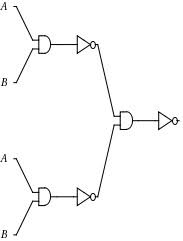
\includegraphics[scale=1]{orwithand.jpg} 
\end{center}


\item A kilobyte is 1024 bytes.How many message can it store?
\[2^{1024} = 179,769,313,486,231,590,772,930,...,304,835,356,329,624,224,137,216 \ digits=39\]
\item What is the entropy associated with the tossing of a fair coin?
\[ H(x) =-\sum_{i=1}^{n} P_{i} \log_{2} P_{i} \] 
We known that information is
\[I = - \log_{2} P_{i}\] 
Then we can write entrophy equation as
\[ H(x) =-\sum_{i=1}^{n} P_{i} I_{i} \]

for tossing of a fair coin

\[ H(x) =- \frac{1}{2} \log_{2} \frac{1}{2} - \frac{1}{2} \log_{2} \frac{1}{2}  = \frac{1}{2} * \frac{1}{2}= 1\] 

\item Suppose that $X$ consist of characters $A$,$B$,$C$,$D$ that occur in a signal with respective probabilities $0.1$,$0.4$,$0.25$ and $0.25$. What is the Shannon entrophy?

\[ H(x) =-\sum_{i=1}^{n} P_{i} \log_{2} P_{i} \] 

\[ H(x) =- 0.1 \log_{2} 0.1 - 0.4 \log_{2}  0.4 - 0.25 \log_{2} 0.25 - 0.25 \log_{2} 0.25  = 1.86096\] 



\item A room full of people has incomes distributed in the follow way:

\begin{itemize}
\item $n(25.5) = 3$
\item $n(30) = 5$
\item $n(42) = 7$
\item $n(50) = 3$
\item $n(63) = 1$
\item $n(75) = 2$
\item $n(90) = 1$
\end{itemize}

What is the most probable income?

\[ n(42) = 7\]

What is the average income?

\[E(x) = 25.5 (\frac{3}{22})+ 30 (\frac{5}{22})+ 42 (\frac{7}{22})+ 50 (\frac{3}{22})+ 63 (\frac{1}{22})+ 75 (\frac{2}{22})+ 90 (\frac{1}{22})= 44.25\] 

What is the variance of this distribution?

\[<j^2> = 25.5^2 (\frac{3}{22})+ 30^2 (\frac{5}{22})+ 42^2 (\frac{7}{22})+ 50^2 (\frac{3}{22})+ 63^2 (\frac{1}{22})+ 75^2 (\frac{2}{22})+ 90^2 (\frac{1}{22})= 2255.35\]

\[ <(\Delta j)^2> = <j^2> - <j>^2 = 297.29 \]
\end{enumerate}









%\end{multicols}
\end{document}